%----------------------------------------------------------------------------------------
%	PACKAGES AND OTHER DOCUMENT CONFIGURATIONS
%----------------------------------------------------------------------------------------
\documentclass[10pt,letterpaper,sans]{moderncv/moderncv} % Font sizes: 10, 11, or 12; paper sizes: a4paper, letterpaper, a5paper, legalpaper, executivepaper or landscape; font families: sans or roman

\moderncvtheme[red]{banking}
% CV color - options include: 'blue' (default), 'orange', 'green', 'red', 'purple', 'grey' and 'black'
% CV theme - options include: 'casual' (default), 'classic', 'oldstyle' and 'banking'

\usepackage[utf8]{inputenc}

\usepackage[top=1cm, bottom=1cm, left=2cm, right=2cm]{geometry} % Reduce document margins
\recomputelengths

\usepackage{fontawesome}

\usepackage{lipsum} % Used for inserting dummy 'Lorem ipsum' text into the template
%\setlength{\hintscolumnwidth}{3cm} % Uncomment to change the width of the dates column
%\setlength{\makecvtitlenamewidth}{10cm} % For the 'classic' style, uncomment to adjust the width of the space allocated to your name

\newcommand{\COMMITHASH}{GITHUBCOMMITHASH}
\newcommand{\RUNNUMBER}{GITHUBRUNNUMBER}


\renewcommand{\phonesymbol}{\faicon{phone}\ }
\renewcommand{\emailsymbol}{\faicon{envelope}\ }
\renewcommand{\addresssymbol}{\faicon{location-arrow}\ }
\renewcommand{\mobilesymbol}{\faicon{mobile}\ }
\renewcommand{\homepagesymbol}{\faicon{link}\ }

%----------------------------------------------------------------------------------------
%	NAME AND CONTACT INFORMATION SECTION
%----------------------------------------------------------------------------------------

\firstname{Giordon} % Your first name
\familyname{Stark} % Your last name

% All information in this block is optional, comment out any lines you don't need
\title{Cover Letter}
\address{Giordon Stark}{223 Arroyo Seco}{Santa Cruz, CA\,\,\,95060} % street, city, country
%\mobile{(302) 584 3464}
%\phone{(000) 111 1112}
%\fax{(000) 111 1113}
\email{kratsg@gmail.com}
\homepage{giordonstark.com}
\extrainfo{\footnotesize Built \href{https://github.com/kratsg/faculty-statements/actions/runs/\RUNNUMBER}{\today}\ from \href{https://github.com/kratsg/faculty-statements/tree/\COMMITHASH}{\faicon{github}@\COMMITHASH}}
%\photo[70pt][0.4pt]{pictures/me.jpg} % The first bracket is the picture height, the second is the thickness of the frame around the picture (0pt for no frame)
%\quote{Some quote}

\makeatletter
\renewcommand*{\makeletterclosing}{
  \@closing\\[0.5em]%
  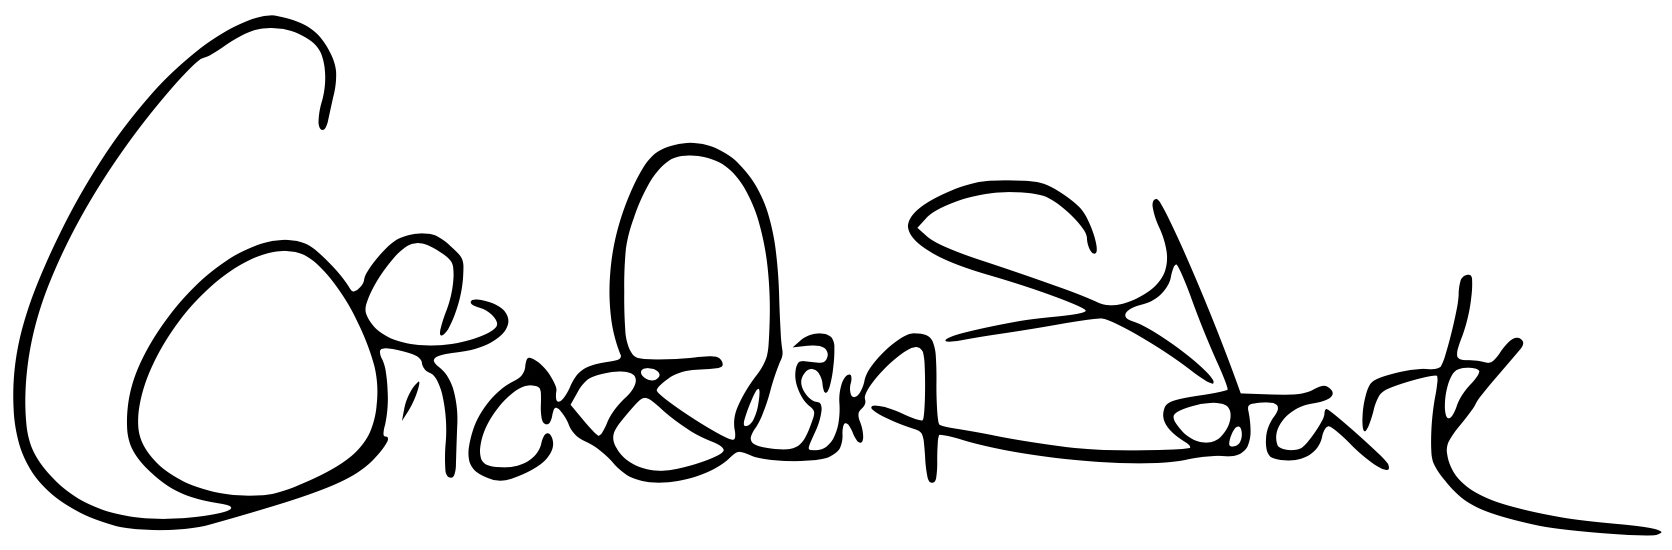
\includegraphics[height=1cm]{pictures/signature}\\% Insert signature
  {\bfseries \@firstname~\@lastname} (pronouns: he/him/point)%
  \ifthenelse{\isundefined{\@enclosure}}{}{%
    \\%
    \vfill%
    {\color{color2}\itshape\enclname: \@enclosure}}}
\makeatother

%----------------------------------------------------------------------------------------

\begin{document}

\recipient{Honeycomb.io}{548 Market Street \#25362\\San Francisco, CA 94104-54013}
\date{March 31st, 2022}
\opening{To whom it may concern,}
\closing{Sincerely,}
\enclosure[Enclosed]{resume}

\makelettertitle
\vspace*{-1em}

Hi Honeycomb.io, you've created quite the... buzz. My name is Giordon Stark, and I am what you might call a "licensed quantum mechanic." Over the past decade, I have spent my time in academia trying to balance the trifecta of work that rattles my hive: physics, software, and hardware. As you have probably guessed by this cover letter and the following resume, I am looking to transition from academia into the tech industry, and you caught my eye. I would best fit a superposition of a data scientist and software engineer role.

In late-2014, I jumped headfirst into a 5000-person international collaboration of physicists, scientists, engineers, students, technicians working on the ATLAS detector at CERN. The first thing I did was start on a problem that needed a solution: design hardware that continues to allow scientists to record data from the experiment in 2022+ using state-of-the-art technology that didn't exist yet! The final design was a single PCB with four FPGAs that could process 40TB/s. This project is gFEX, a "global" Feature EXtractor, recently installed in the detector. It's not perfect, I will admit, but like Dune, the physics must flow. Being fast and close to right is better than being perfect. The engineers and scientists I collaborated with knew we had a limited budget and a limited timeline, so our focus was to ensure that very few iterations on the design were needed while being cheap enough to produce another electronic board as required.

At the same time as my hardware work, I worked on physics analyses, searching for signs of new physics. Along this avenue, I built up my management and leadership experience. I took on a leadership role in the analysis my Ph.D. thesis is on, and this came with some fascinating politics working in a large team. In ATLAS, everyone who spends a year contributing to the experiment qualifies as an author, which means their name is allowed to be on papers published by the collaboration. This authorship policy also means that you circulate it internally for review when you have an analysis complete and your paper written up. Everyone has a say in what your plots look like, your uncertainty estimation, and whether your color choices insult their sensibilities. I learned an important lesson - feedback is a gift. The publication procedure put in place exposed me to ideas, experiences, and perspectives that I appreciate as it allows me to be a better physicist and human bee-ing. Coordinating the analysis teams gives me the bigger picture to understand the human impact on physics and how crucial it is to make sure that nobody feels like they take a backseat in their analysis.

And of course, last but not least, the third branch of my work ethic is software. I treat software as a skill that everyone deserves access to obtain. I spent a significant amount of effort helping pull our entire collaboration out of the dark shade of Subversion to Git and GitLab. I was happy to bring my three-hour crash course on GitLab CI/CD to a larger audience as part of Software Carpentry. I teach newcomers about empowerment and ownership of their code, the conscientiousness of the software they develop and maintain. Why? As a team, we have a responsibility to make sure continuity happens. If an early-career scientist needs to take a break, perhaps because of a war in their country, I want those folks not to feel pressured by work obligations. Those with the privilege can step in, provide support, and help carry on. With this mindset, I spend my time developing tools to improve the experience of the analyzers and engineers, inspired in part by the frustration I deal with during my daily work.

In short, I believe that I am an adult with many questions that would be a good fit for your company, able to pick up new skills and handle steep learning curves. There are plenty of other unique and quirky skills that I cannot include in a short cover letter or resume, such as baking or finding bugs in systems. But isn't that what people say? You catch more bugs with honey[comb.io] than vinegar.

\makeletterclosing
\end{document}
